\objectives{%
  \item implement gradient descent for any given loss function and (usually)
       thereby automatically and efficiently find nearly-optimal linear
       hypotheses from data
}

%\samquote{
%  Hey Jude, don't make it bad \\
%  Take a sad song and make it better \\
%  Remember to let her under your skin \\
%  Then you'll begin to make it \\
%  Better, better, better, better, better, better, ...
%}{paul mccartney, john lennon}

        %-- gradients
        %-- writing out the code : a key exercise ; batches
        %-- setting initialization and learning rate; local minima
        %-- visualizing noise and curvature

\sampassage{(stochastic) gradient descent}
  We seek a hypothesis that is best (among a class $\hH$) according to some
  notion of how well each hypothesis models given data:
  \begin{lstlisting}[language=Python, basicstyle=\footnotesize\ttfamily]
    def badness(h,y,x):
        # return e.g. whether h misclassifies y,x OR h's surprise at seeing y,x OR etc
    def badness_on_dataset(h, examples):
        return np.mean([badness(h,y,x) for y,x in examples])
  \end{lstlisting}
        %#return np.mean([for y,x in examples])

  %For example, out notion of goodness might map $h$ to its
  %training accuracy $1-\Ein$.  Or, when $h$ has a probabilistic interpretation,
  %our notion of goodness might map $h$ to the probability it predicts for the
  %training outputs $y_i$.\bovinenote{%
  %  In either case, we view our notion-of-good, computed on the training data,
  %  as an estimate of the notion-of-good we most care about: testing
  %  performance.  So $1-\Ein$ estimates $1-\Eout$ and $p(y_i|x_i;h)$ for $y_i,
  %  x_i$ a training example estimates $p(y|x;h)$ for $y,x$ fresh data.
  %}
  %
  Earlier we found a nearly best candidate by brute-force search over all
  hypotheses.  But this doesn't scale to most interesting cases wherein $\hH$
  is intractably large.
  %
  So: \emph{what's a faster algorithm to find a nearly best candidate?}

  A common idea is to start arbitrarily with some $h_0\in \hH$ and
  repeatedly improve to get $h_1, h_2, \cdots$.  We eventually stop, say at $h_{10000}$.
  The key question is:\bovinenote{%
    Also important are the questions of where to start and when to stop.
    But have patience!  We'll discuss these later.
  }
  \emph{how do we compute an improved hypothesis $h_{t+1}$ from our current
  hypothesis $h_t$}?

  We \emph{could} just keep randomly nudging $h_t$ until we hit on an
  improvement; then we define $h_{t+1}$ as that improvement.  Though this
  sometimes works surprisingly well,\bovinenote{%
    If you're curious, search `metropolis hastings' and
    `probabilistic programming'.
  } we can often save time by exploiting more available information.
  Specifically, we can inspect $h_t$'s inadequacies to inform our proposal
  $h_{t+1}$.
  %
  Intuitively, if $h_t$ misclassifies a particular $(x_i, y_i) \in \sS$, then
  we'd like $h_{t+1}$ to be like $h_t$ but nudged toward
  accurately classifying $(x_i, y_i)$.\bovinenote{%
    In doing better on the $i$th datapoint, we might mess up how we do
    on the other datapoints!  We'll consider this in due time.
  }

  How do we compute ``{a nudge toward accurately classifying $(x, y)$}''?  That
  is, how do measure how slightly changing a parameter affects some result?
  Answer: derivatives!  To make $h$ less bad on an example $(y, x)$, we'll
  nudge $h$ in tiny bit along $-g = -d \texttt{badness}(h,y,x) /
  dh$. Say, $h$ becomes $h-0.01g$.\bovinenote{%
    E.g.\ if each $h$ is a vector and we've chosen
    $\texttt{badness}(h,y,x) = -y h\cdot x$ as our notion of badness, then $-d
    \texttt{badness}(h,y,x) / dh = +yx$, so we'll nudge $h$ in the
    direction of $+yx$.
    \exercise{Is this update familiar?}
  }
  Once we write
  \begin{lstlisting}[language=Python, basicstyle=\footnotesize\ttfamily]
    def gradient_badness(h,y,x):
        # returns the derivative of badness(h,y,x) with respect to h
    def gradient_badness_on_dataset(h, examples):
        return np.mean([gradient_badness(h,y,x) for y,x in examples])
  \end{lstlisting}
  we can repeatedly nudge via \textbf{gradient descent (GD)}, the engine of ML:\bovinenote{%
    \noparexercise{Can GD directly minimize misclassification rate?}
  }
  \begin{lstlisting}[language=Python, basicstyle=\footnotesize\ttfamily]
    h = initialize()
    for t in range(10000):
      h = h - 0.01 * gradient_badness_on_dataset(h, examples)
  \end{lstlisting}
  Since the derivative of total badness depends on all the training data,
  looping $10000$ times is expensive.  So in practice we estimate the needed
  derivative based on some \emph{subset} (jargon: \textbf{batch}) of the
  training data --- a different subset each pass through the loop --- in what's
  called \textbf{stochastic gradient descent (SGD)}:
  \begin{lstlisting}[language=Python, basicstyle=\footnotesize\ttfamily]
    h = initialize()
    for t in range(10000):
      batch = select_subset_of(examples)
      h = h - 0.01 * gradient_badness(h, batch)
  \end{lstlisting}
  \begin{marginfigure}[-0cm]
    \centering
    \picturew{0.99\textwidth}{gradients-curvy.png}%
    \caption{%
      An intuitive picture of gradient descent.  Vertical axis is training loss
      and the other two axes are weight-space.
      %
      Warning: though logistic loss (and the L2 regularizer) is smooth,
      perceptron and hinge loss (and the L1 regularizer) have jagged angles or
      `joints'.  Also, all five of those functions are convex.
      %
      %But the picture above is smooth and nonconvex.
      %
      The smooth, nonconvex picture here is most apt for deep learning (Unit
      3).
    }
    \attnsam{cartoon of GD}
  \end{marginfigure}

  (S)GD requires informative derivatives.  Misclassification rate has
  uninformative derivatives: any tiny change in $h$ won't change the predicted
  labels.  But when we use probabilistic models, small changes in $h$ can lead
  to small changes in the predicted \emph{distribution} over labels.
  %
  To speak poetically: the softness of probabilistic models paves a smooth ramp
  over the intractably black-and-white cliffs of `right' or `wrong'.
  %
  We now apply SGD to maximizing probabilities.

\sampassage{maximum likelihood estimation}
  When we can compute each hypothesis $h$'s asserted probability
  that the training $y$s match the training $x$s, it seems
  reasonable to seek an $h$ for which this probability is maximal.  This
  method is \textbf{maximum likelihood estimation (MLE)}.
  %
  It's convenient for the overall goodness to be a sum (or average) over each
  training example.  But independent chances multiply rather than add:
  rolling snake-eyes has chance $1\!/\!6 \cdot 1\!/\!6$, not $1\!/\!6 + 1\!/\!6$.  So
  we prefer to think about maximizing log-probabilities instead of maximizing
  probabilities --- it's the same in the end.\bovinenote{%
    Throughout this course we make a crucial assumption that our training
    examples are independent from each other.
  }
  By historical
  convention we like to minimize badness rather than maximize goodness, so
  we'll use SGD to \emph{minimize negative-log-probabilities}.
  \begin{lstlisting}[language=Python, basicstyle=\footnotesize\ttfamily]
    def badness(h,y,x):
        return -np.log( probability_model(y,x,h) )
  \end{lstlisting}

  Let's see this in action for the linear logistic model we developed for soft
  binary classification.  A hypothesis $\vec w$ predicts that a (featurized)
  input $\vec x$ has label $y=+1$ or $y=-1$ with chance $\sigma(+ \vec w \cdot \vec x)$
  or $\sigma(- \vec w \cdot \vec x)$:
  $$
    p_{\sfy|\sfx,\sfw}(y|\vec x,\vec w) = \sigma(y \vec w \cdot \vec x)
    \quad\quad
    \text{where}
    \quad\quad
    \sigma(\frd) = 1/(1-\exp(-\frd))
  $$
  So MLE with our logistic model means finding $\vec w$ that \emph{minimizes}
  $$
    -\log\wrap{\text{prob of all $y_i$s given all $\vec x_i$s and $\vec w$}}
    =
    \sum_i -\log(\sigma(y_i \vec w\cdot \vec x_i))
  $$
  The key computation is the derivative of those badness terms:\bovinenote{%
    Remember that $\sigma\pr(z) = \sigma(z)\sigma(-z)$.
    %
    To reduce clutter we'll temporarily write $y \vec w\cdot \vec x$ as $ywx$.
  }
  $$
    \frac{\partial (-\log(\sigma(y w x)))}{\partial w}
    =
    \frac{-\sigma(y w x)\sigma(-y w x) y x}{\sigma(y w x)}
    =
    - \sigma(-y w x) y x
  $$

  \exercise{If you're like me, you might've zoned out by now.  But this stuff
  is important, especially for deep learning!  So please graph the
  above expressions to convince yourself that our formula for derivative
  makes sense visually.}

  \vspace{\baselineskip}

  To summarize, we've found the loss gradient for the logistic model:
  \begin{lstlisting}[language=Python, basicstyle=\footnotesize\ttfamily]
    sigma = lambda z : 1./(1+np.exp(-z))
    def badness(w,y,x):             return -np.log( sigma(y*w.dot(x)) )
    def gradient_badness(w,y,x):    return -sigma(-y*w.dot(x)) * y*x
  \end{lstlisting}
  As before, we define overall badness on a dataset as an average badness over
  examples; and for simplicity, let's intialize gradient descent at $h_0=0$:
  \begin{lstlisting}[language=Python, basicstyle=\footnotesize\ttfamily]
    def gradient_badness_on_dataset(h, examples):
      return np.mean([gradient_badness(h,y,x) for y,x in examples])
    def initialize():
        return np.zeros(NUMBER_OF_DIMENSIONS, dtype=np.float32)
  \end{lstlisting}
  Then we can finally write gradient descent:
  \begin{lstlisting}[language=Python, basicstyle=\footnotesize\ttfamily]
    h = initialize()
    for t in range(10000):
      h = h - 0.01 * gradient_badness_on_data(h, examples)
  \end{lstlisting}

  %\attnsam{mention convexity and convergence?}

  \begin{marginfigure}[-5cm]
    \centering
    \picturew{0.99\textwidth}{gd-problem.png}\\%
    \picturew{0.99\textwidth}{gd-answers.png}%
    \caption{%
        \noparexercise{%
        Shown is a small training set (originally $1$-D but featurized using
        the bias trick) and our current weight vector.
        Here {\blu blue} is the positive label.
        \emph{Which direction will
        the weight vector change if we do one step of (full-batch) gradient
        descent?} Four options are shown; one is correct.
        }
    \attnsam{caption}
    }
  \end{marginfigure}



  \begin{marginfigure}
     \attnsam{show trajectory in weight space over time -- see how certainty
  degree of freedom is no longer redundant? (``markov'')}\\
    \attnsam{show training and testing loss and acc over time}
  \end{marginfigure}




%#-------  _  ------------------------------------------------------------------


  \newpage
\sampassage{least-squares regression}
  We've been focusing on classification.  Regression is the same story.
  %Briefly, we want to maximize thdata terms $\ell(y_k, w\cdot x_k)$ plus
  %an implausibility term $\lambda w\cdot w / 2$.  Whereas with (say, logistic)
  Instead of logistic probabilities we have gaussian probabilities.  So
  we want to minimize\bovinenote{%
    \noparexercise{%
      Suppose all the training points $x_k$ are the same, say $(1, 0) \in \Rr^2$.
      What's the $w$ optimal according to the above loss?
    }
  } this loss (here, $\varphi(x)$ represents the feature vector for raw input $x$):
  $$
    \lambda w\cdot w/2
    + \sum_k (y_k - w\cdot \varphi(x_k))^2/2
  $$
  instead of minimizing a classifier loss such as
  $
    \lambda w\cdot w/2
    + \sum_k \log(1/\sigma(y_k w\cdot \varphi(x_k)))
  $.\bovinenote{%
    Compare those two losses when
    $(y_k, w\cdot \varphi(x_k)) = (+1, +10)$ or
    $(-1, +10)$.
  }
  We can do this by gradient descent.
  \attnsam{y-d heatmaps of logistic vs gaussian!}
  \attnsam{contour maps showing that $\lambda$ does not merely scale}

  However, in this case we can write down the answer in closed form.  This gives us qualitative insight.
  (In
  practice our fastest way to evaluate that closed form formula \emph{is} by
  fancy versions of gradient descent!)
  %
  We want\bovinenote{%
    \noparexercise{%
      Verify that the gradient (with respect to $w$) of the above loss is
      $$
        \lambda w - \sum_k (y_k - w\cdot \varphi(x_k)) \varphi(x_k)
      $$
      If $\lambda=0$ and $w\cdot \varphi(x_k)$ overestimates $y_k$, which way
      would a gradient update on the $k$th training example change $w$?  Is
      this intuitive?
    }
  }
  $$
    0 = \lambda w - \sum_k (y_k - w\cdot \varphi(x_k)) \varphi(x_k)
  $$
  Since $(w\cdot \varphi(x_k)) \varphi(x_k) = \varphi(x_k) \varphi(x_k)^T w$, we have
  $$
    \sum_k y_k \varphi(x_k) = \wrap{\lambda \, \text{Id} + \sum_k \varphi(x_k) \varphi(x_k)^T} w
  $$
  or
  $$
    w = \wrap{\lambda \, \text{Id} + \sum_k \varphi(x_k) \varphi(x_k)^T}^{-1} \wrap{\sum_k y_k \varphi(x_k)}
  $$
  Let's zoom way out:\bovinenote{%
    \noparexercise{%
      Fix some training set.  Consider the optimal weight $w_\star$ as a
      function of our regularization strength $\lambda$.  How does 
      the regularization value $\lambda w_\star\cdot w_\star/2$ change as we
      increase $\lambda$?
    }
  } neglecting that we can't divide by vectors and neglecting
  $\lambda$, we read the above as saying that $w = (x^2)^{-1}(yx) = y/x$; this
  looks right since $w$ is our ideal exchange rate from $x$ to $y$!  The $\lambda$
  makes that denominator a bit bigger: $w = (\lambda + x^2)^{-1}(yx) = y/(x+\lambda/x)$.
  A bigger denominator means a smaller answer, so $\lambda$ pulls $w$ toward
  $0$.  Due to the $x$s in the denominator, $\lambda$ has less effect --- it pulls $w$ less ---
  for large $x$s.  This is because large $x$s have `more leverage', i.e. are
  more constraining evidence on what $w$ ought to be.
  %This reflects that \attnsam{--- prior vs likelihood; leverage!}

  \begin{figure}%[-0cm]
    \centering
    %\picturew{0.85\textwidth}{regression-beach.png}%
    \picturew{0.65\textwidth}{regress-springs.png}%
    \caption{%
      Here's an illuminating physical analogy.
      %
      The least-squares loss says we want decision function values $d$ to be
      close to the true $y$s.  So we can imagine hooking up a stretchy {\blu
      spring} from each {\rng training point $(x_i, y_i)$} to our
      \textbf{predictor line (or hyperplane)}.  Bolt that line to the origin,
      but let it rotate freely.  The springs all want to have zero length.
      Then minimizing least-squares loss is the same as minimizing potential
      energy!
      %
      We can also model L2 regularizers, which say that the predictor line wants to be
      horizontal.  So we tie a \textbf{special (black) spring} from the
      input-space (say, at $x=1$) to the line.  The larger the L2's $\lambda$,
      the stiffer this spring is compared to the others.
      %
      To get this to fully work, we need to keep all the springs vertical.
      (The mechanically inclined reader might enjoy imagining joining together
      a pair of slippery sheaths, one slipping along the predictor line and the
      other slipping along a fixed vertical pole.)
      %
      Then the analogy is mathematically exact.
      %
      \attnsam{TODO EXPAND ON THIS CAPTION!}
    }
  \end{figure}
  \exercise{%
    Momentarily neglect $\lambda$.  Visualize one gradient update on the
    spring figure above: is the torque clockwise or anti-clockwise?
    Now, is there some value of $\lambda$ for which the springs are in static
    equilibrium?
  }
  \exercise{%
    True or false: the most stretched-out (blue) spring contributes the
    greatest non-regularizer term to the loss gradient?
  }

  %TODO \attnsam{Exercise: James Stein}
  %TODO \attnsam{Illustration: (nonlinear $\varphi$ --- mushrooms)}

%#-------  _  ------------------------------------------------------------------
%#-------  _  ------------------------------------------------------------------
%#-------  _  ------------------------------------------------------------------
%#-------  _  ------------------------------------------------------------------


  \newpage
\sampassage{initialization, learning rate, local minima}\marginnote{\veryoptional}

\sampassage{pictures of training: noise and curvature}\marginnote{\veryoptional}
  \par\attnsam{}
  \par\attnsam{}
  \par\attnsam{test vs train curves: overfitting}
  \par\attnsam{random featurization: double descent}

\sampassage{practical implementation: vectorization}


%    \samsection{5. ideas in optimization}
%      \samquote{
%        premature optimization is the root of all evil
%      }{donald knuth}
%
%        \attn{learning rate as metric; robustness to 2 noise structures}
%        \attn{nesterov momentum}
%        \attn{decaying step size; termination conditions}
%        \attn{batch normalization}
%
%
%
%%~~~~~~~~~~~~~~~~~~~~~~~~~~~~~~~~~~~~~~~~~~~~~~~~~~~~~~~~~~~~~~~~~~~~~~~~~~~~~~
%%~~~~~~~~~~~~~  2.20. local minima  ~~~~~~~~~~~~~~~~~~~~~~~~~~~~~~~~~~~~~~~~~~~
%
%      \sampassage{local minima}
%        % convexity, initialization
%
%%~~~~~~~~~~~~~~~~~~~~~~~~~~~~~~~~~~~~~~~~~~~~~~~~~~~~~~~~~~~~~~~~~~~~~~~~~~~~~~
%%~~~~~~~~~~~~~  2.21. implicit regularization  ~~~~~~~~~~~~~~~~~~~~~~~~~~~~~~~~
%
%      \sampassage{implicit regularization}
%
%%~~~~~~~~~~~~~~~~~~~~~~~~~~~~~~~~~~~~~~~~~~~~~~~~~~~~~~~~~~~~~~~~~~~~~~~~~~~~~~
%%~~~~~~~~~~~~~  2.22. learning rate schedule  ~~~~~~~~~~~~~~~~~~~~~~~~~~~~~~~~~
%
%      \sampassage{learning rate schedule}
%
%%~~~~~~~~~~~~~~~~~~~~~~~~~~~~~~~~~~~~~~~~~~~~~~~~~~~~~~~~~~~~~~~~~~~~~~~~~~~~~~
%%~~~~~~~~~~~~~  2.23. learning rates as dot products  ~~~~~~~~~~~~~~~~~~~~~~~~~
%
%      \sampassage{learning rates as dot products} % connects to whitening / pre-conditioning; ties into next section on kernels
%
%


  %\begin{marginfigure}[-0cm]
  %  \centering
  %  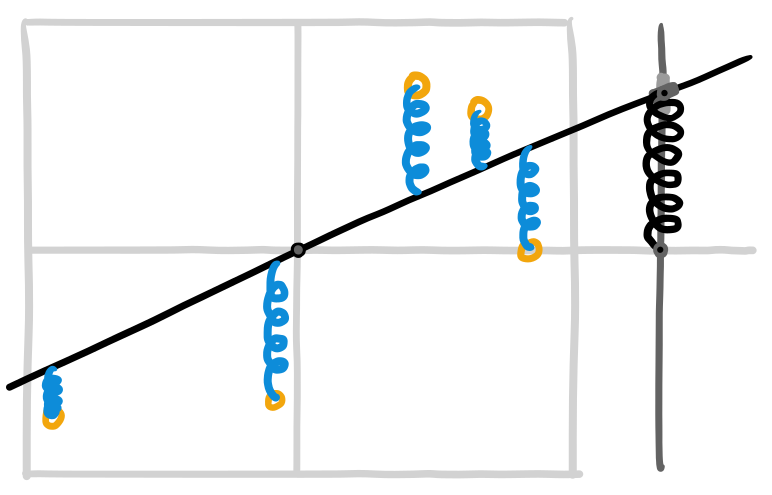
\includegraphics[width=0.99\textwidth]{./regress-springs.png}
  %  \caption{%
  %  \attnsam{caption}
  %  }
  %\end{marginfigure}

  %\begin{marginfigure}[-0cm]
  %  \centering
  %  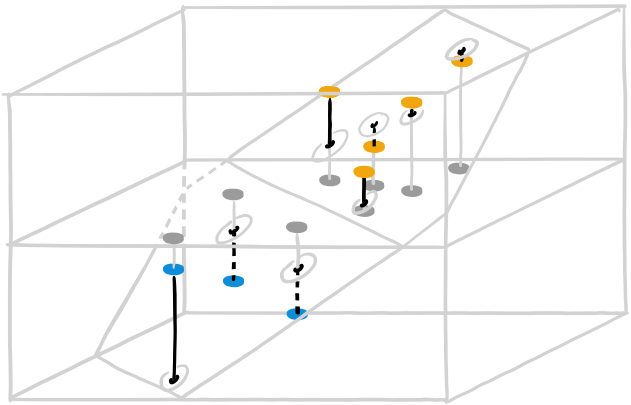
\includegraphics[width=0.99\textwidth]{./regression-beach.png}
  %  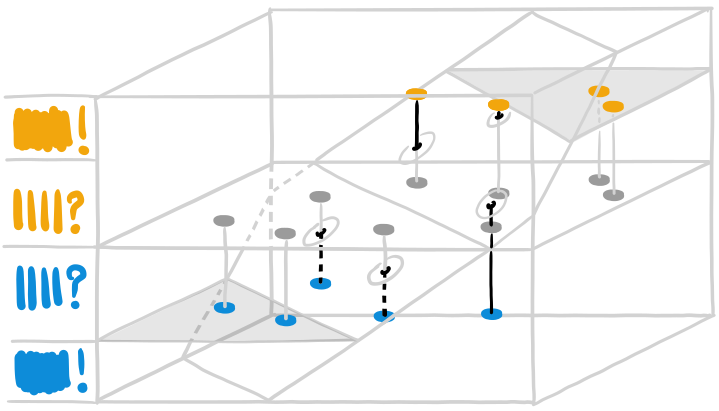
\includegraphics[width=0.99\textwidth]{./hinge-beach.png}
  %  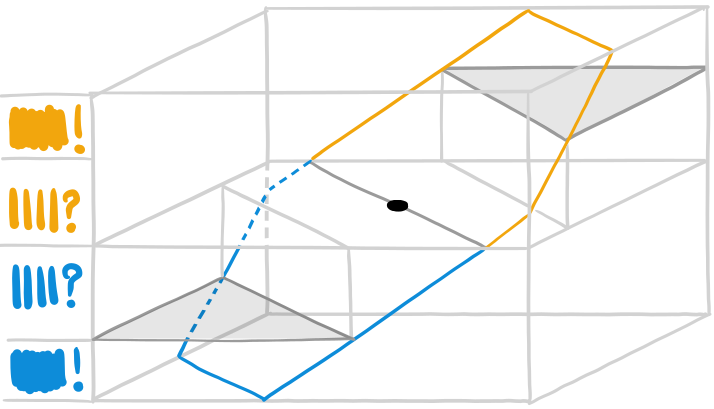
\includegraphics[width=0.99\textwidth]{./beach.png}
  %  \caption{%
  %  \attnsam{caption}
  %  }
  %\end{marginfigure}
